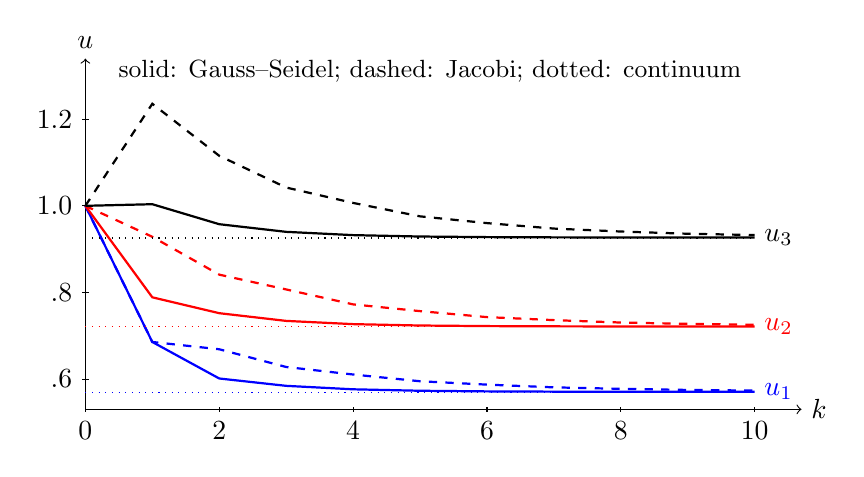
\begin{tikzpicture}[x=.85cm,y=5.5cm]
\draw[->] (0,.53)--(10.7,.53) node[right] {$k$};
\draw[->] (0,.53)--(0,1.34) node[above] {$u$};
\draw[blue,thick,dashed] plot coordinates {(0.000000,1.000000) (1.000000,0.685619) (2.000000,0.668787) (3.000000,0.627836) (4.000000,0.610505) (5.000000,0.594936) (6.000000,0.587145) (7.000000,0.580837) (8.000000,0.577435) (9.000000,0.574853) (10.000000,0.573385)};
\draw[blue,thick] plot coordinates {(0.000000,1.000000) (1.000000,0.685619) (2.000000,0.601303) (3.000000,0.584336) (4.000000,0.576334) (5.000000,0.572964) (6.000000,0.571530) (7.000000,0.570921) (8.000000,0.570662) (9.000000,0.570552) (10.000000,0.570505)};
\draw[blue,dotted] (0,0.5690826)--(10,0.5690826);
\node[blue,right] at (10,0.5704701) {$u_1$};
\draw[red,thick,dashed] plot coordinates {(0.000000,1.000000) (1.000000,0.928466) (2.000000,0.841101) (3.000000,0.806930) (4.000000,0.772450) (5.000000,0.756853) (6.000000,0.743033) (7.000000,0.736106) (8.000000,0.730499) (9.000000,0.727475) (10.000000,0.725180)};
\draw[red,thick] plot coordinates {(0.000000,1.000000) (1.000000,0.788741) (2.000000,0.752098) (3.000000,0.734295) (4.000000,0.726819) (5.000000,0.723637) (6.000000,0.722284) (7.000000,0.721709) (8.000000,0.721465) (9.000000,0.721361) (10.000000,0.721317)};
\draw[red,dotted] (0,0.7204917)--(10,0.7204917);
\node[red,right] at (10,0.7212840) {$u_2$};
\draw[black,thick,dashed] plot coordinates {(0.000000,1.000000) (1.000000,1.235619) (2.000000,1.115516) (3.000000,1.042258) (4.000000,1.006731) (5.000000,0.975681) (6.000000,0.960089) (7.000000,0.947475) (8.000000,0.940671) (9.000000,0.935506) (10.000000,0.932570)};
\draw[black,thick] plot coordinates {(0.000000,1.000000) (1.000000,1.003736) (2.000000,0.957558) (3.000000,0.939923) (4.000000,0.932342) (5.000000,0.929122) (6.000000,0.927753) (7.000000,0.927171) (8.000000,0.926924) (9.000000,0.926818) (10.000000,0.926774)};
\draw[black,dotted] (0,0.9257815)--(10,0.9257815);
\node[black,right] at (10,0.9267407) {$u_3$};
\foreach \k in {0,2,4,6,8,10} \draw (\k,.535)--(\k,.525) node[below] {$\k$};
\foreach \v in {.6,.8,1.0,1.2} \draw (.05,\v)--(-.05,\v) node[left] {$\v$};
\node[anchor=west,font=\small] at (.35,1.31) {solid: Gauss--Seidel; dashed: Jacobi; dotted: continuum};
\end{tikzpicture}
